\section{Architettura}\label{sec:mooncloud-archi}

\begin{figure}
	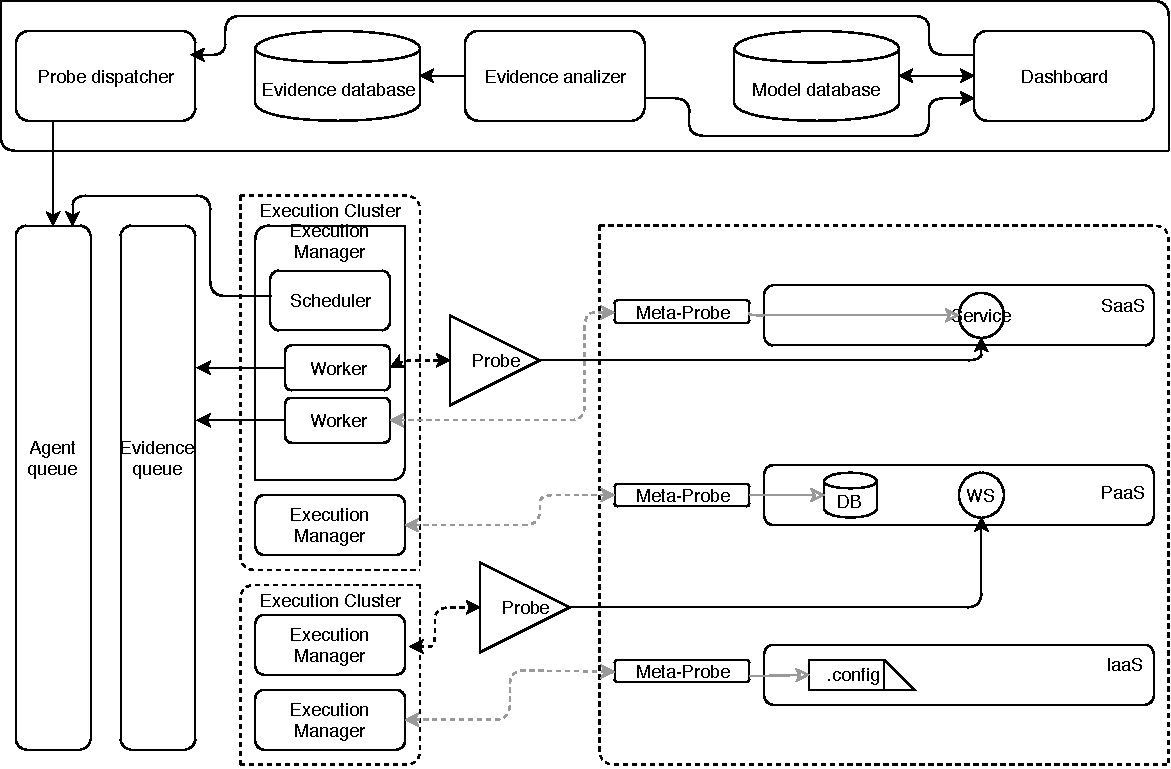
\includegraphics[scale=0.6]{img/mooncloud_archi}
	\caption{L'architettura di MoonCloud}
	\label{fig:mooncloud-archi-fig}
\end{figure}

Logicamente, è possibile dividere l'architettura MoonCloud
in due macrocomponenti, così come mostrato in figura \ref{fig:mooncloud-archi-fig}.
La comunicazione tra di essi avviene mediante due code:
\begin{description}
	\item[\texttt{Agent Queue}]Su di essa vengono inviate richieste di esecuzione di test.
	\item[\texttt{Evidence Queue}]E' responsabile del passaggio delle evidenze tra
	il componente di esecuzione e quello di gestione. 
\end{description}
I due macrocomponenti sono:
\begin{description}
	\item[\texttt{Certification Manager}]Si occupa dell'orchestrazione
	dell'intero processo di certificazione. Ne fanno parte i seguenti moduli:
	\begin{itemize}
		\item \texttt{Dashboard}: una web GUI utilizzata dai clienti per
		      gestire l'intero processo di certificazione
		\item \texttt{Model Database}: una base di dati in cui sono memorizzate
		      tutte le regole relative al processo di certificazione (e di verifica
		      dei modelli)
		\item \texttt{Probe Dispatcher} il quale si occupa della comunicazione
		      tra \texttt{Certification Manager} ed i cluster di esecuzione.
		\item \texttt{Result Database} ovvero una base di dati
		\texttt{InfluxDB} in
		      cui vengono salvate le evidenze collezionate durante i test\footnote{\url{https://www.influxdata.com/}}
		\item \texttt{Evidence Analyzer} è un componente responsabile di analizzare
		      le evidenze raccolte nella specifica base di dati. % e di verificare la correttezza di modelli.
	\end{itemize}
	\item[\texttt{Execution Cluster}]Un set di VM dedicate all'esecuzione dei
	test così come orchestrato dal \texttt{Certification Manager}. In ciascun
	cluster vi sono uno o più \texttt{Execution Manager}, responsabili
	della gestione degli agent per l'analisi. Ognuno di questi \texttt{Manager}
	è composto da:
	\begin{itemize}
		\item \texttt{Scheduler}: aspetta richieste dal \texttt{Certification Manager}
		      e ne fa il dispatching al successivo componente.    
		\item \texttt{Worker}: esso è connesso direttamente agli agenti che analizzano,
		      manda ad essi le configurazioni necessarie, ne raccoglie le evidenze e le invia
		      al \texttt{Certification Manager}.
	\end{itemize}
\end{description}

Gli agent di esecuzione a loro volta si dividono in due categorie:
\begin{description}
	\item[\texttt{Probe}]Sono responsabili dell'esecuzione dei test e del
	monitoraggio in un certo ToC.
	\item[\texttt{Meta-probe}]Si occupano di verificare eventuali violazioni ai
	vincoli di tempo, probabilità, configurazioni. 
\end{description}
Si può dire che mentre il primo tipo di \textit{probe} sia \textit{invasivo}, il secondo invece
ha un minore overhead in quanto si limita a verificare una certa proprietà
senza interferire con il normale funzionamento del sistema.
Poiché prevedono una forma di analisi meno intrusiva, il minor overhead comporta
anche una minore qualità delle evidenze raccolte.
Ad esempio, un \textit{probe} potrebbe utilizzare \texttt{nmap} per verificare che
una certa comunicazione sia cifrata con TLS, mentre un \textit{meta-probe} si
potrebbe limitare a leggere un file di configurazione alla ricerca dell'opzione
che abiliti la cifratura TLS.

Entrambi sono eseguiti come dei container \textit{Docker} su delle \textit{Docker machine}
(ci si riferirà ad esse anche come \textit{Docker host}),
e si dispone anche di un repository interno di ricette per essi\footnote{\url{https://www.docker.com/}}.
L'attività di test è eseguita da script Python all'interno di questi container.
L'utilizzo di Docker ha un grande vantaggio: mediante i \texttt{Dockerfile} si possono
specificare tutte le dipendenze necessarie ad un certo test, le quali saranno
installate automaticamente in fase di creazione dell'immagine. Non è quindi necessario
preoccuparsi di avere una piattaforma di esecuzione sui cui siano disponibili \textit{tutte}
le dipendenze che servono.

D'ora in poi ci si riferirà al termine ``\textit{rete MoonCloud}'' come a quella
delle costituita dalle Docker machine e dal relativo \texttt{Execution Cluster}.